\section{Construcción del corpus}

\subsection{Extracción}
\begin{frame}
    \frametitle{Extracción}

    \begin{itemize}
        \item Humorístico: se busca en Twitter por la palabra clave \emph{chistes} y se eligen cuentas, llegando a 16.488 tweets.
        \item No humorístico: cuentas de noticias, frases filosóficas y curiosidades, alcanzando los 22.875 tweets.
    \end{itemize}
\end{frame}

\subsection{Anotación}
\begin{frame}
    \frametitle{Anotación}

    \begin{itemize}
        \item Naturalmente se etiquetarían los tweets según su tipo de cuenta; pero se encuentran inconsistencias.

        \begin{itemize}
            \item Hay que anotarlos a mano.
        \end{itemize}

        \item Excesiva cantidad de tweets para anotar.

        \begin{itemize}
            \item Se crea una aplicación para que usuarios los anoten.
        \end{itemize}
    \end{itemize}

    \vspace{1cm}

    \begin{center}
        \bf
        Los usuarios definen al humor.
    \end{center}
\end{frame}

\begin{frame}
\frametitle{Anotación}
\framesubtitle{Aplicación Final}
    \begin{center}
        \begin{columns}[c]
            \begin{column}[c]{0.45\textwidth}
                \centering
                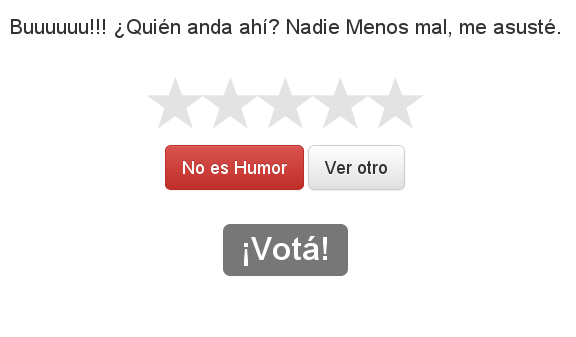
\includegraphics[frame, height=3.5cm]{pagina.png}
            \end{column}

            \begin{column}[c]{0.45\textwidth}
                \centering
                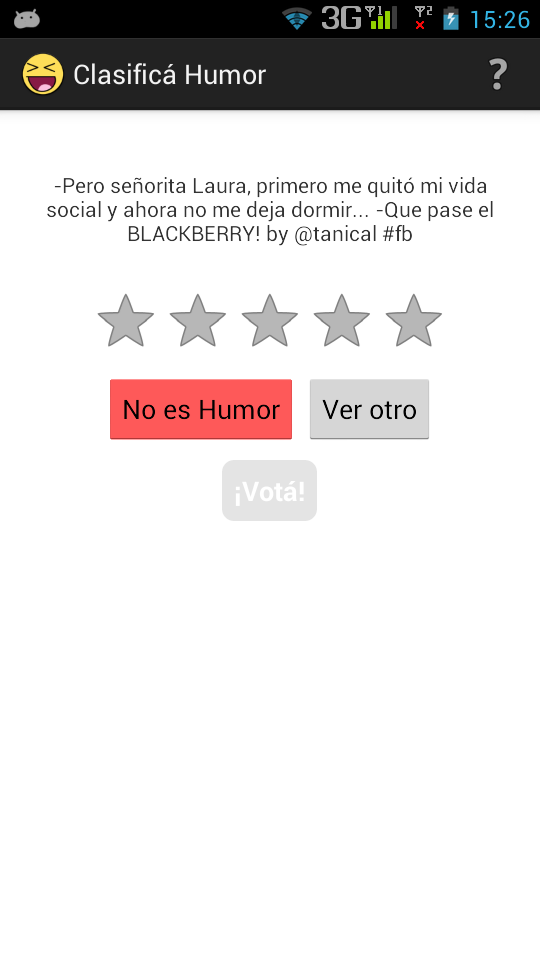
\includegraphics[frame, height=7cm]{app.png}
            \end{column}
        \end{columns}
    \end{center}
\end{frame}

\subsubsection{Resultado de la anotación}
\begin{frame}[allowframebreaks]
    \frametitle{Resultado de la anotación}

    \begin{itemize}
        \item[+] 60k votaciones recibidas
        \item[--] 20k votaciones eliminadas
        \item[--] 6,5k votaciones “ver otro” (\emph{“skip”})
        \item[=] 33,5k votos considerados
    \end{itemize}

    \framebreak

    \begin{center}
        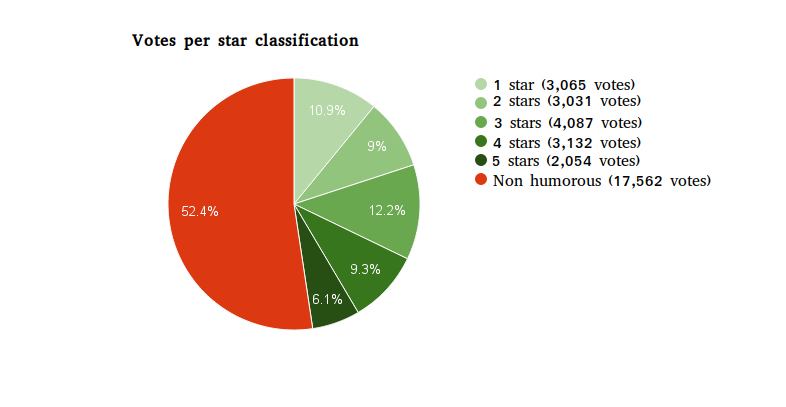
\includegraphics{votos_por_calificacion_torta.png}

        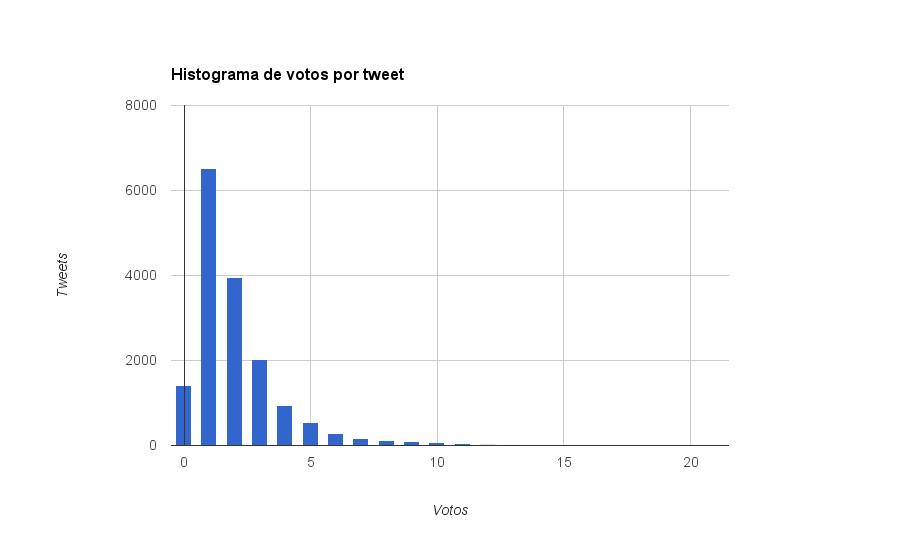
\includegraphics{histograma.png}
    \end{center}
\end{frame}

\subsubsection{Humor según la votación}

\begin{frame}[allowframebreaks]
    \frametitle{Humor según la votación}

    Porcentaje de votos positivos: $\frac{\#\{votos\ positivos\}}{\#\{total\ votos\}}$

    \begin{center}
        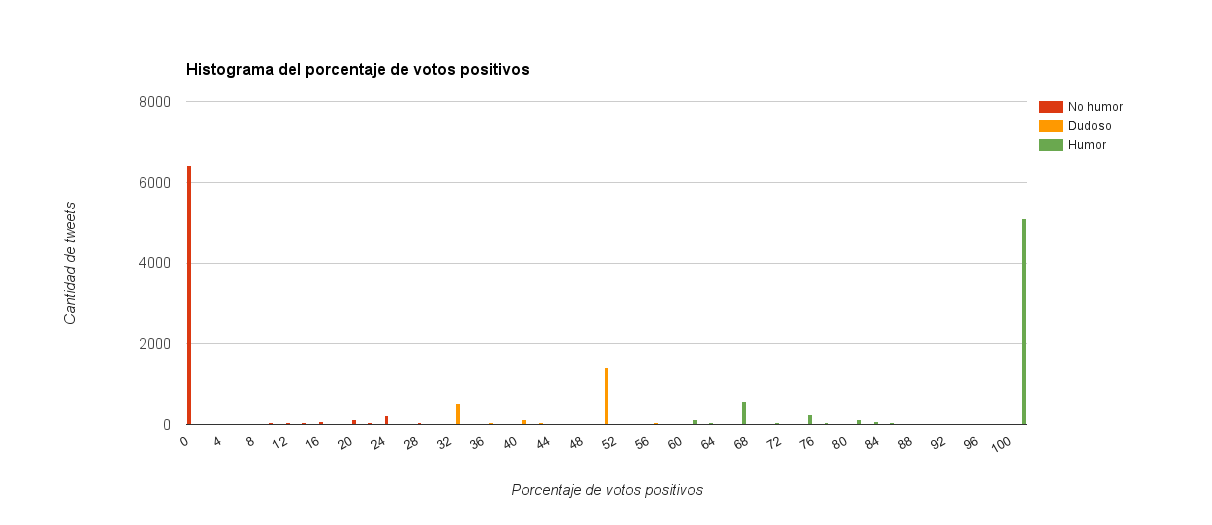
\includegraphics[height=3.75cm]{histograma_porcentaje_humor.png}
    \end{center}

    \begin{itemize}
        \item $[60\%, 100\%] \Rightarrow$ \textbf{Humor}
        \item $(30\%, 60\%) \Rightarrow$ \textbf{Dudoso}
        \item $[0\%, 30\%] \Rightarrow$ \textbf{No humor}
    \end{itemize}

    \framebreak

    \begin{center}
        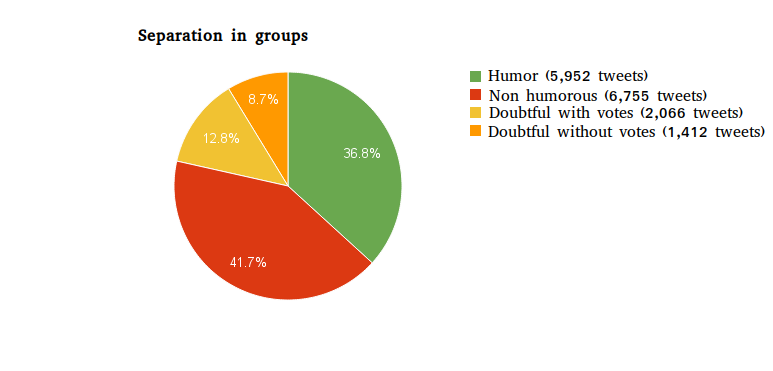
\includegraphics[height=6.5cm]{grupos.png}
    \end{center}
\end{frame}
